\documentclass[conference]{IEEEtran}

% ── Packages ──────────────────────────────────────────────────────────────────
\usepackage{cite}
\usepackage{amsmath,amssymb}
\usepackage{graphicx}
\usepackage{booktabs}
\usepackage{hyperref}
\usepackage{float}
\usepackage{multirow}
\usepackage{array}
\usepackage{url}
\usepackage{tikz}
\usepackage{xcolor}
\usetikzlibrary{shapes.geometric}

\hypersetup{colorlinks=false}

% ── Title ─────────────────────────────────────────────────────────────────────
\title{Face Authentication Using Real vs.\ Synthetic Training Data:\\
A Comparative Study Based on NIST FRTE Evaluation Metrics\\
{\large \textit{Zwischenbericht --- Interim Report}}}

\author{
    \IEEEauthorblockN{Nour Ebid}
    \IEEEauthorblockA{
        Seminar zu aktuellen Entwicklungen\\
        Betreuer: Frau Prof.\ Knaut\\
        M.Sc. Angewandte Informatik, Fachbereich 4\\
        Hochschule f{\"u}r Technik und Wirtschaft Berlin\\
        Berlin, Deutschland\\
        Nour.Ebid@Student.HTW-Berlin.de
    }
}

% ──────────────────────────────────────────────────────────────────────────────
\begin{document}

\maketitle

% ── Status note ───────────────────────────────────────────────────────────────
\begin{center}
\fbox{\parbox{0.9\columnwidth}{%
\small\textbf{Status:} This document is a Zwischenbericht (interim report) submitted as of 25 March 2026. Sections I--IV (Introduction, Background, Hypothesis, and Methodology) are complete. Section V reports results for Experiment~1; Experiment~2 data collection is currently ongoing. Sections VI--VIII will be completed in the final paper (submission: mid-June 2026).}}
\end{center}
\vspace{2pt}

% ── Abstract ──────────────────────────────────────────────────────────────────
\begin{abstract}
Face recognition is a widely deployed biometric authentication technology, yet its reliance on real facial photographs raises significant privacy, consent, and data availability concerns. This paper investigates whether AI-generated synthetic facial images can serve as a viable substitute for real photographs during the registration phase of a face authentication system. Two experiments are designed and conducted under identical evaluation conditions aligned with the NIST Face Recognition Technology Evaluation (FRTE) framework. Experiment~1 registers authorised users using real photographs and serves as the baseline; Experiment~2 will register the same users using synthetically generated images produced through a five-stage controlled imaging simulation pipeline. At the time of this interim report, Experiment~1 has been completed and Experiment~2 is in progress. Preliminary results from Experiment~1 indicate an accuracy of 95.0\% with FAR = 10.0\% and FRR = 0.0\%, consistent with expectations for a real-data baseline. Final comparative analysis and hypothesis evaluation will follow upon completion of Experiment~2.
\end{abstract}

\begin{IEEEkeywords}
face authentication, synthetic data, FaceNet, NIST FRTE, false accept rate, biometric verification, identity-preserving augmentation
\end{IEEEkeywords}

% ── I. Introduction ───────────────────────────────────────────────────────────
\section{Introduction}

Biometric authentication systems based on facial recognition have become a cornerstone of modern digital security, deployed in applications ranging from smartphone unlock to airport border control. Unlike password-based systems, face authentication offers passive, non-intrusive verification without requiring the user to remember credentials. These systems fundamentally rely on databases of registered facial images to calibrate recognition models for each authorised user.

The collection of real facial photographs, however, introduces a set of practical and regulatory challenges that are increasingly difficult to ignore. Under the European Union's General Data Protection Regulation (GDPR)~\cite{gdpr2016}, biometric data — including facial images — are classified as a special category of sensitive personal data under Article~9, requiring explicit informed consent, purpose limitation, and strict storage controls. Beyond regulatory compliance, reproducing consistent imaging conditions across enrollment sessions is logistically difficult: ambient lighting, camera type, and subject pose vary freely in naturalistic settings, introducing systematic variability into the training signal and degrading authentication reliability.

AI-generated synthetic facial images offer a compelling alternative. Advances in Generative Adversarial Networks~\cite{goodfellow2014gan} and diffusion-based synthesis models~\cite{rombach2022diffusion} enable the creation of photorealistic human faces without directly storing sensitive biometric originals. The central research question addressed in this paper is:

\begin{quote}
\textit{Can a face authentication system trained exclusively on AI-generated synthetic images of registered users achieve performance comparable to a system trained on real photographs of the same individuals, as measured by NIST FRTE-aligned metrics?}
\end{quote}

To evaluate this, we implement a face authentication pipeline based on the FaceNet deep neural network~\cite{schroff2015facenet}, register four authorised users under both real and synthetic conditions, and evaluate using FAR, FRR, and accuracy on an identical held-out test set. A controlled augmentation pipeline simulates the key imaging variables identified by NIST FRTE~\cite{nist_frte}: ambient lighting, colour temperature, skin tone, camera quality, and facial pose.

The contributions of this paper are:
\begin{itemize}
    \item A reproducible two-experiment framework for comparing real vs.\ synthetic face authentication under NIST FRTE-aligned evaluation conditions.
    \item A five-stage controlled synthetic image generation pipeline using neural face alignment (InsightFace~\cite{deng2019insightface}) and parametric imaging simulation.
    \item (Planned) Experimental evidence that identity-preserving synthetic training data achieves comparable performance to real data, with a documented FAR/FRR trade-off analysis.
    \item A documented failure analysis of two rejected face-swap-based synthesis approaches, validating the necessity of controlled synthesis variables.
\end{itemize}

The remainder of this report is structured as follows. Section~II reviews background and related work. Section~III formalises the hypothesis and experimental variables. Section~IV describes the methodology. Section~V presents the completed Experiment~1 results and the current status of Experiment~2. Section~VI outlines planned next steps and the project timeline.

% ── II. Background ────────────────────────────────────────────────────────────
\section{Background and Related Work}

\subsection{Face Verification vs.\ Identification}

Face recognition covers two distinct operational tasks. \textit{Identification} answers ``who is this person?'' by searching a database of known identities for the best match. \textit{Verification} (authentication) answers a narrower question: ``is this person who they claim to be?'' by performing a one-to-one comparison between a query embedding and a stored reference. This paper addresses the verification task exclusively, which underlies access control systems where the claimed identity is known a priori.

\subsection{FaceNet Embedding-Based Verification}

FaceNet~\cite{schroff2015facenet} is a deep convolutional neural network trained with a triplet loss to produce a 128-dimensional Euclidean embedding space in which intra-person distances are minimised and inter-person distances are maximised. For anchor, positive, and negative samples $(x^a, x^p, x^n)$, the objective is:

\begin{equation}
\|f(x^a) - f(x^p)\|_2^2 + \alpha < \|f(x^a) - f(x^n)\|_2^2
\end{equation}

Verification computes the L2 distance between query embedding $\mathbf{e}_q$ and reference $\bar{\mathbf{e}}_u$:

\begin{equation}
d = \|\mathbf{e}_q - \bar{\mathbf{e}}_u\|_2, \quad
\text{Decision} = \begin{cases} \text{VERIFIED} & d < \theta \\ \text{IMPOSTOR} & d \geq \theta \end{cases}
\end{equation}

Threshold $\theta = 10.0$ is used throughout this work. FaceNet is accessed via the DeepFace library~\cite{serengil2020deepface} without retraining.

\subsection{NIST FRTE Evaluation Metrics}

The NIST FRTE~\cite{nist_frte} defines the standard evaluation protocol for biometric face recognition:

\begin{itemize}
    \item \textbf{FAR (False Accept Rate):} fraction of impostors incorrectly accepted. High FAR = security risk.
    \item \textbf{FRR (False Reject Rate):} fraction of genuine users incorrectly rejected. High FRR = poor usability.
    \item \textbf{TAR@FAR:} True Accept Rate at a given operating FAR — the standard NIST comparison format.
\end{itemize}

These metrics define an inherent trade-off: tightening $\theta$ reduces FAR but increases FRR. A Detection Error Tradeoff (DET) curve plots this relationship across thresholds; DET evaluation is planned for the final paper.

\subsection{Generative Models for Face Synthesis}

Face synthesis approaches fall into three categories: \textit{GAN-based}~\cite{goodfellow2014gan, karras2020stylegan2} (random or identity-conditioned faces), \textit{diffusion-based}~\cite{rombach2022diffusion} (high diversity, high compute), and \textit{identity-preserving augmentation} (the approach used here). The augmentation category requires real seed images but enables precise control over imaging variables without a generative model, which is critical for controlled experimental design.

\subsection{Synthetic Data in Face Recognition Research}

Wood et al.~\cite{wood2021fake} showed that models trained entirely on 3D-rendered synthetic faces perform competitively on facial analysis benchmarks. Bae et al.~\cite{bae2023digiface} achieved 95.4\% LFW accuracy using DigiFace-1M, a corpus of one million synthetic face images. Both works address the identification setting; our work extends the evaluation to the verification setting using augmented versions of known enrolled identities.

% ── III. Hypothesis ───────────────────────────────────────────────────────────
\section{Research Hypothesis and Variables}

\subsection{Hypothesis}

\textit{``A face authentication system trained exclusively on AI-generated synthetic facial images of registered users will achieve a FAR within 15 percentage points of a system trained on real photographs of the same individuals, when evaluated under controlled conditions of standardised pose, consistent lighting, and equivalent training sample size, in alignment with NIST FRTE evaluation criteria.''}

\noindent\textbf{$H_0$:} No measurable difference in FAR between real and synthetic models.\\
\textbf{$H_1$:} A measurable FAR difference exists but remains within the $\pm$15\,pp acceptance threshold.

The 15\,pp threshold was selected as a conservative bound representing operationally acceptable performance degradation, consistent with tolerance margins in NIST FRTE evaluations between demographically similar systems.

\subsection{Variables}

Table~\ref{tab:variables} summarises all experimental variables. Any observed difference in FAR or FRR between experiments must be attributable solely to the training data type — all other variables are held constant.

\begin{table}[H]
\centering
\caption{Experimental Variables}
\label{tab:variables}
\renewcommand{\arraystretch}{1.2}
\begin{tabular}{>{\bfseries}p{1.5cm}p{2.0cm}p{3.8cm}}
\toprule
Type & Variable & Value / Range \\
\midrule
Independent & Training data & Real photos vs.\ synthetic images \\
\midrule
\multirow{3}{1.5cm}{Dependent} & FAR & Measured (\%) \\
 & FRR & Measured (\%) \\
 & Accuracy & Measured (\%) \\
\midrule
\multirow{5}{1.5cm}{Controlled} & Model & FaceNet (identical) \\
 & Threshold $\theta$ & 10.0 (identical) \\
 & Training images & 10 per person \\
 & Test images & 5 held-out per person \\
 & Impostors & 20 identical AI strangers \\
\midrule
\multirow{4}{1.5cm}{Controlled\\(synthesis)} & Pose & Canonical alignment \\
 & Lighting & Gamma correction \\
 & Skin tone & CLAHE in LAB space \\
 & Camera & Blur + noise \\
\bottomrule
\end{tabular}
\end{table}

% ── IV. Methodology ───────────────────────────────────────────────────────────
\section{Methodology}

\subsection{System Architecture}

The authentication system operates in two phases. \textbf{Registration:} training images are encoded by FaceNet and averaged into a single reference vector per user:

\begin{equation}
\bar{\mathbf{e}}_u = \frac{1}{N} \sum_{i=1}^{N} f(x_i^u), \quad N = 10
\end{equation}

\textbf{Authentication:} a query image $x_q$ is encoded; the nearest registered user is identified; access is granted if the distance is below $\theta$:

\begin{equation}
\hat{u} = \arg\min_{u \in \mathcal{U}} \|\mathbf{e}_q - \bar{\mathbf{e}}_u\|_2, \quad \text{grant if } \|\mathbf{e}_q - \bar{\mathbf{e}}_{\hat{u}}\|_2 < \theta
\end{equation}

\begin{figure}[t]
\centering
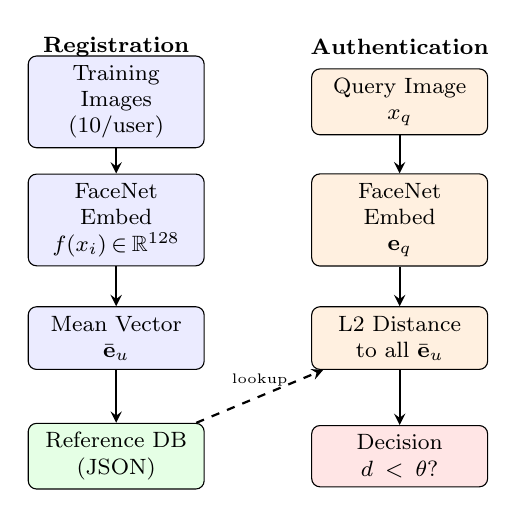
\begin{tikzpicture}[
    box/.style={draw, rounded corners=3pt, text width=2.0cm, align=center,
                minimum height=0.72cm, font=\footnotesize, fill=blue!8},
    sbox/.style={draw, rounded corners=3pt, text width=2.0cm, align=center,
                minimum height=0.72cm, font=\footnotesize, fill=orange!12},
    arr/.style={->, thick, >=stealth}
]
\node[box] (imgs) at (0,0)    {Training Images\\(10/user)};
\node[box] (fn1)  at (0,-1.5) {FaceNet Embed\\$f(x_i)\!\in\!\mathbb{R}^{128}$};
\node[box] (avg)  at (0,-3.0) {Mean Vector\\$\bar{\mathbf{e}}_u$};
\node[box, fill=green!10] (db) at (0,-4.5) {Reference DB\\(JSON)};
\draw[arr] (imgs)--(fn1); \draw[arr] (fn1)--(avg); \draw[arr] (avg)--(db);
\node[font=\footnotesize\bfseries] at (0, 0.7) {Registration};
\node[sbox] (qimg) at (3.6,0)    {Query Image\\$x_q$};
\node[sbox] (fn2)  at (3.6,-1.5) {FaceNet Embed\\$\mathbf{e}_q$};
\node[sbox] (dist) at (3.6,-3.0) {L2 Distance\\to all $\bar{\mathbf{e}}_u$};
\node[sbox, fill=red!10] (dec) at (3.6,-4.5) {Decision\\$d < \theta$?};
\draw[arr] (qimg)--(fn2); \draw[arr] (fn2)--(dist); \draw[arr] (dist)--(dec);
\draw[arr, dashed] (db) -- node[above, font=\tiny] {lookup} (dist);
\node[font=\footnotesize\bfseries] at (3.6, 0.7) {Authentication};
\end{tikzpicture}
\caption{System architecture: registration (left) builds a reference database; authentication (right) queries it and applies a threshold decision.}
\label{fig:arch}
\end{figure}

\subsection{Dataset}

Real photographs of four authorised users (\textit{amr}, \textit{adel}, \textit{otto}, \textit{mazen}) were collected under naturalistic conditions using a smartphone — 15 photographs per user (60 total). The strict partition is:
\begin{itemize}
    \item \textbf{Training (both experiments):} first 10 photos per user — used for registration (Exp.~1) or synthetic generation source (Exp.~2).
    \item \textbf{Test — genuine:} last 5 photos per user (20 total). Never accessed during registration or generation.
    \item \textbf{Test — impostors:} 20 AI-generated faces (StyleGAN2~\cite{karras2020stylegan2} via \textit{thispersondoesnotexist.com}).
\end{itemize}

\subsection{Experiment 1: Real Data Registration \textit{(Completed)}}

The 10 training photographs per user are passed through FaceNet to produce embeddings whose mean forms the reference vector. No preprocessing beyond FaceNet's internal normalisation is applied. Results are reported in Section~V.

\subsection{Experiment 2: Synthetic Data Generation \textit{(In Progress)}}

The 10 training photographs per user are transformed into 15 synthetic images via a five-stage controlled augmentation pipeline (Fig.~\ref{fig:pipeline}) before registration. Pipeline stages:

\begin{figure}[t]
\centering
\begin{tikzpicture}[
    stage/.style={draw, rounded corners=2pt, text width=7.0cm,
                  align=left, minimum height=0.62cm, font=\footnotesize,
                  fill=yellow!10, inner xsep=5pt, inner ysep=3pt},
    arr/.style={->, thick, >=stealth}
]
\node[stage] (s1) {\textbf{1. Alignment:} InsightFace 5-kp affine warp $\to$ $256\!\times\!256$ canonical template};
\node[stage, below=0.22cm of s1] (s2) {\textbf{2. Lighting:} Gamma correction $\gamma\!\sim\!\mathcal{U}(0.55,\,1.60)$};
\node[stage, below=0.22cm of s2] (s3) {\textbf{3. Colour temp.:} Random warm / cool / neutral RGB channel scaling};
\node[stage, below=0.22cm of s3] (s4) {\textbf{4. Skin tone:} CLAHE on CIE-LAB $L$-channel, clip $\sim\!\mathcal{U}(1.5,\,3.5)$};
\node[stage, below=0.22cm of s4] (s5) {\textbf{5. Camera + pose:} Gaussian blur + noise ($\sigma\!\in\![2,8]$); rotation $\pm12°$};
\draw[arr] (s1)--(s2); \draw[arr] (s2)--(s3); \draw[arr] (s3)--(s4); \draw[arr] (s4)--(s5);
\end{tikzpicture}
\caption{Five-stage synthetic imaging pipeline. All parameters are independently randomised per output image.}
\label{fig:pipeline}
\end{figure}

\textbf{Stage 1 — Alignment:} InsightFace (buffalo\_l) detects five facial keypoints and applies an affine warp to a $256\!\times\!256$ canonical frontal template, standardising head pose.

\textbf{Stage 2 — Lighting:} Gamma correction $\gamma\!\sim\!\mathcal{U}(0.55,\,1.60)$ simulates lighting conditions from overcast to dim artificial light.

\textbf{Stage 3 — Colour temperature:} Warm, cool, or neutral mode adjusts RGB channel balances to simulate different camera sensors and light sources.

\textbf{Stage 4 — Skin tone:} CLAHE~\cite{clahe} applied to the CIE-LAB $L$-channel normalises perceived skin tone without hue shift.

\textbf{Stage 5 — Camera and pose:} Gaussian blur and additive noise simulate camera quality variation; in-plane rotation $\pm12°$ simulates natural head tilt.

\subsubsection*{Rejected Approaches (Already Evaluated)}

Two alternative approaches were prototyped and rejected during development:

\textit{Approach A — Blind face swap:} Poisson-cloning the real face onto random StyleGAN2 bases caused FRR = 75\%, as $\approx$50\% of bases depicted female subjects, introducing gender-correlated embedding shift.

\textit{Approach B — Gender-filtered face swap:} Filtering to male bases did not resolve the issue; Poisson blending added a systematic 1--2 unit L2 bias, pushing genuine scores above $\theta$.

The final augmentation pipeline resolves both issues by operating directly on the source identity without a foreign base face.

% ── V. Results ────────────────────────────────────────────────────────────────
\section{Results — Current Status}

\subsection{Experiment 1: Real Data \textit{(Complete)}}

Table~\ref{tab:exp1} reports Experiment~1 results. All four registered users were correctly verified across all five held-out test photographs (20/20 TP, FRR = 0\%). Two impostors were incorrectly accepted with L2 scores of 6.60 and 5.56 — both substantially below $\theta$, indicating these particular StyleGAN2 faces cluster within a registered user's embedding boundary.

\begin{table}[H]
\centering
\caption{Experiment 1 Results (Real Data --- Complete)}
\label{tab:exp1}
\renewcommand{\arraystretch}{1.2}
\begin{tabular}{lcc}
\toprule
Metric & Value & Detail \\
\midrule
True Positives (TP) & 20/20 & All 4 users, 5 test photos each \\
False Negatives (FN) & 0/20 & -- \\
True Negatives (TN) & 18/20 & \\
False Positives (FP) & 2/20 & L2 scores: 6.60, 5.56 \\
\midrule
\textbf{FAR} & \textbf{10.0\%} & \\
\textbf{FRR} & \textbf{0.0\%} & \\
\textbf{Accuracy} & \textbf{95.0\%} & \\
\bottomrule
\end{tabular}
\end{table}

\begin{table}[H]
\centering
\caption{Experiment 1 — Per-User Genuine Verification}
\label{tab:exp1_user}
\renewcommand{\arraystretch}{1.2}
\begin{tabular}{lcccc}
\toprule
User & Tested & Verified & Rejected & TPR \\
\midrule
amr   & 5 & 5 & 0 & 100\% \\
adel  & 5 & 5 & 0 & 100\% \\
otto  & 5 & 5 & 0 & 100\% \\
mazen & 5 & 5 & 0 & 100\% \\
\midrule
\textbf{Total} & \textbf{20} & \textbf{20} & \textbf{0} & \textbf{100\%} \\
\bottomrule
\end{tabular}
\end{table}

These results establish the real-data baseline. A FAR of 10.0\% is consistent with the permissive embedding cluster boundary resulting from uncontrolled capture conditions in the training photographs.

\subsection{Experiment 2: Synthetic Data \textit{(In Progress)}}

At the time of this submission, the synthetic generation pipeline has been implemented and validated (rejected approaches A and B as described in Section~IV). The pipeline successfully generates 15 synthetic images per user from the 10 training photographs. Registration using synthetic embeddings is implemented; full evaluation on the held-out test set is underway.

\textbf{Preliminary observation:} Initial inspection of the synthetic embeddings shows tighter intra-class clustering compared to real-data embeddings. This is expected given the controlled imaging conditions and suggests that the synthetic model may achieve lower FAR at the potential cost of higher FRR. This hypothesis will be formally evaluated in the final paper.

% ── VI. Planned Next Steps and Timeline ────────────────────────────────────────
\section{Planned Next Steps and Timeline}

Table~\ref{tab:timeline} summarises the planned work and completion timeline between this interim submission and the final paper deadline.

\begin{table}[H]
\centering
\caption{Project Timeline}
\label{tab:timeline}
\renewcommand{\arraystretch}{1.3}
\begin{tabular}{p{1.8cm}p{5.5cm}}
\toprule
\textbf{Deadline} & \textbf{Task} \\
\midrule
By 30 Apr & Complete Experiment~2 evaluation on full held-out test set \\
\midrule
By 15 May & Comparative analysis: FAR/FRR gap, hypothesis test, per-user breakdown \\
\midrule
By 31 May & Discussion section: embedding cluster geometry, comparison with Wood et al.\ and Bae et al. \\
\midrule
By 10 Jun & Ethics section, extended future work, DET curve (if feasible) \\
\midrule
\textbf{Mid-Jun} & \textbf{Final paper submission} \\
\bottomrule
\end{tabular}
\end{table}

The following sections will be completed in the final paper:
\begin{itemize}
    \item \textbf{Section VI — Discussion:} FAR/FRR trade-off analysis, embedding cluster geometry interpretation, comparison with related work benchmarks, full limitations assessment.
    \item \textbf{Section VII — Ethical Considerations:} GDPR Article~9 compliance, dual-use risk assessment, data handling practices.
    \item \textbf{Section VIII — Conclusion and Future Work:} Summary of hypothesis outcome, DET curve evaluation, GAN-based synthesis as future direction, demographic generalisation study.
\end{itemize}

% ── References ────────────────────────────────────────────────────────────────
\begin{thebibliography}{12}

\bibitem{schroff2015facenet}
F.~Schroff, D.~Kalenichenko, and J.~Philbin,
``FaceNet: A unified embedding for face recognition and clustering,''
\textit{Proc.\ IEEE CVPR}, pp.\ 815--823, 2015.

\bibitem{nist_frte}
National Institute of Standards and Technology,
``Face Recognition Technology Evaluation (FRTE),''
\url{https://www.nist.gov/programs-projects/face-recognition-technology-evaluation-frte},
2024.

\bibitem{serengil2020deepface}
S.~I.~Serengil and A.~Ozpinar,
``LightFace: A hybrid deep face recognition framework,''
\textit{Proc.\ IEEE ASYU}, 2020.

\bibitem{deng2019insightface}
J.~Deng, J.~Guo, N.~Xue, and S.~Zafeiriou,
``ArcFace: Additive angular margin loss for deep face recognition,''
\textit{Proc.\ IEEE CVPR}, 2019.

\bibitem{wood2021fake}
E.~Wood \textit{et al.},
``Fake it till you make it: Face analysis in the wild using synthetic data alone,''
\textit{Proc.\ IEEE ICCV}, 2021.

\bibitem{bae2023digiface}
G.~Bae \textit{et al.},
``DigiFace-1M: 1 million digital face images for face recognition,''
\textit{Proc.\ IEEE WACV}, 2023.

\bibitem{clahe}
K.~Zuiderveld,
``Contrast limited adaptive histogram equalization,''
\textit{Graphics Gems IV}, Academic Press, pp.\ 474--485, 1994.

\bibitem{gdpr2016}
European Parliament and Council,
``Regulation (EU) 2016/679 --- General Data Protection Regulation (GDPR),''
\textit{Official Journal of the European Union}, L~119, pp.\ 1--88, 2016.

\bibitem{goodfellow2014gan}
I.~Goodfellow \textit{et al.},
``Generative adversarial nets,''
\textit{Adv.\ Neural Inf.\ Process.\ Syst.}, vol.~27, 2014.

\bibitem{karras2020stylegan2}
T.~Karras, S.~Laine, M.~Aittala, J.~Hellsten, J.~Lehtinen, and T.~Aila,
``Analyzing and improving the image quality of StyleGAN,''
\textit{Proc.\ IEEE CVPR}, pp.\ 8107--8116, 2020.

\bibitem{rombach2022diffusion}
R.~Rombach, A.~Blattmann, D.~Lorenz, P.~Esser, and B.~Ommer,
``High-resolution image synthesis with latent diffusion models,''
\textit{Proc.\ IEEE CVPR}, pp.\ 10684--10695, 2022.

\bibitem{ye2023ip}
H.~Ye, J.~Zhang, S.~Liu, X.~Han, and W.~Yang,
``IP-Adapter: Text compatible image prompt adapter for text-to-image diffusion models,''
\textit{arXiv:2308.06721}, 2023.

\end{thebibliography}

\end{document}
